\chapter{Conception}

In this section we present the design of the solution built during the
internship with its different components. The main focus was to find a relevant
metric (from \ref{sect:possible_metrics}) to measure the similarity between two
columns, and it is the angular metric that has been used as it takes into
account the magnitude of each point and it responds well to the problem of big
dimensions presented by the euclidean metric, also, it is not limited to measure
similarities over discrete data as the Jaccard similarity does.

The choice of the angular metric implies that the LSH method for the indexation
process has to be chosen from the ones that estimate this metric. We go for
cross-polytope as LSH method to estimate the similarities of the euclidean
metric on a unit sphere (which has the same order of magnitude as the angular
metric).

Our solution is divided into two main parts, the first part is related to the
indexation process where the dataset indexes are computed and stored, and the
second part is meant to take the process of detecting similarities between
datasets through their previously computed indexes.


\section{Indexation}
As described previously, this phase consists of computing the index of each
dataset's column and to store it in a database. This process is completed
through the following three steps:

\subsection{Preprocessing}
The indexes are based on the column types, 2 types are considered: textual
columns and non textual columns (numerical columns). The preprocessing will be
different depending on the column separation process:
\subsubsection{Non-Textual (Numerical) columns}
One of cross-polytope requirements is that the data should have a size equal to
a power of 2, for this we'll set this size on a value between 128 to 2048, and
we'll call it \mbox{DEFAULT\_DATA\_SIZE}.

A random sample of size \mbox{DEFAULT\_DATA\_SIZE} is picked for each column
and then normalized to have the data ready to be indexed with cross-polytope.

\subsubsection{Textual columns}
The textual columns have a different type of preprocessing, it is based on
embedding them with a pre-trained embedding model and a certain approach, the
embedding approach indicates how the embedding model is used over all the cells
to have as a result one vector representing the column content. Four approaches
will be tested to pick the most accurate one.

\paragraph{Approach 1}: The idea of this approach is to concatenate the texts of
each cell to have one text that will be embedded with the chosen embedding
model. The output will depend on this embedding model, and the last step will be
to pad this output with zeros to make it of a size equal to a power of 2.

\paragraph{Approach 2}: This approach consists of embedding each cell on its own
with the chosen embedding model, and then to concatenate this embeddings to form
one vector that will be the output of this approach.

\paragraph{Approach 3}: This approach has the same logic as the previous one, it
adds an extra step which is to perform a PCA on each embedding just before
concatenating in order to have more control over the size of the output and to
make it satisfy the cross-polytope conditions easily.

\paragraph{Approach 4}: This approach also has the same logic of the second one,
meaning that it starts with embedding each cell independently, and then get the
mean of each component of the embedding vector.
\begin{equation}
    a_{i / i \in [1, m]} = \frac{1}{n} \sum_{j=0}^{n} e_{j, i}
\end{equation}
Where:
\begin{multicols}{2}
    \begin{itemize}
        \item $m$ is the size of the embedding model's output.
        \item $n$ is the size of the column.
        \item $e_j$ is the embedding of the $j^{th}$ cell.
        \item $e_{j, i}$ is the $i^{th}$ component of the $j^{th}$ cell
        embedding.
    \end{itemize}
\end{multicols}

The last step in this approach will be to pad this output with zeros to make it
of a size equal to a power of 2.


This step takes as input the concerned dataset, and outputs a list of columns
with their preprocessed data for both textual and non-textual data.

\subsection{Computing index}
At the level of computing indexes, we get the preprocessed column groups and we
pass both of them to the indexation phase by applying Multi-Probe Cross-Polytope
LSH.

Two parameters need to be tuned at this level, the number of hashing functions
to apply by Cross-Polytope LSH, and the number of probes to consider by
Multi-Probe. The choice of these two parameters is explained in section
\ref{chap:exp_and_tests}

This step outputs two groups of indexes, the group of textual column indexes, and
the group of non-textual column indexes. Each column index is represented by an
array of 2 dimensions, where each row represents the result of the corresponding
hashing function, and each column represents an element of the probing sequence
for this hashing function result.

The figure \ref{fig:indexation_process} illustrates the process of preprocessing
and computing the indexes of a dataset.

\begin{figure}[h]
    \centering
    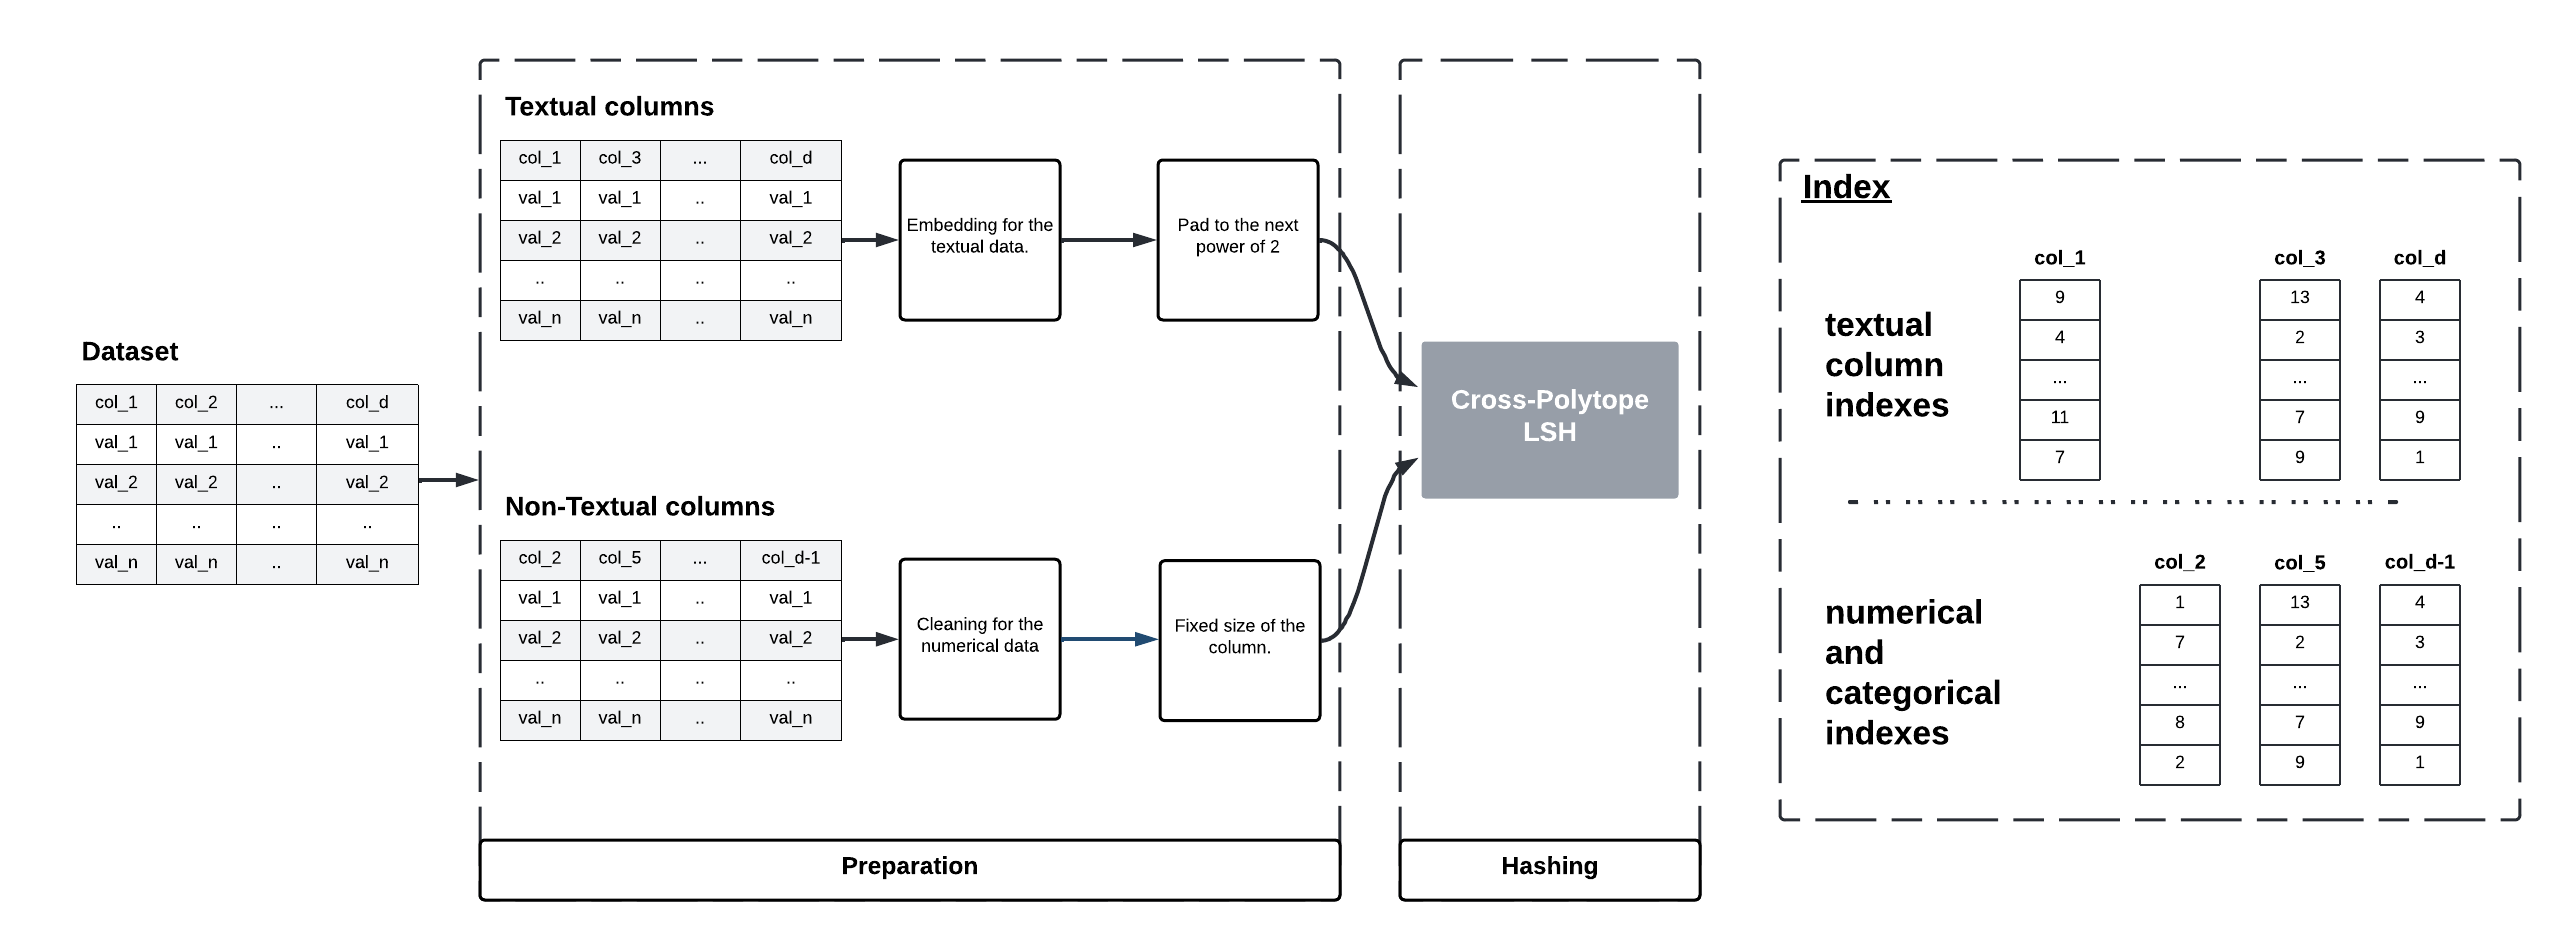
\includegraphics[width=\textwidth]{conception/indexing-whitebg.png}
    \caption{Indexation process illustration}
    \label{fig:indexation_process}
\end{figure}

\subsection{Storing index}
The indexes computed in the previous step need to be stored in order to be used
lately in similarity detection. A key is assigned to every dataset in Talend
Data Inventory, this key is used to store the indexes corresponding to each
dataset. The indexes are stored in a dedicated database which contains the
following attributes:

\begin{itemize}
    \item \textbf{dataset\_id}: Integer. The ID of the corresponding dataset.
    \item \textbf{column\_name}: String. The name of the index column.
    \item \textbf{column\_type}: String. The type of the index column.
    \item \textbf{signature}: Bytes. The encoding of the index.
\end{itemize}


\section{Similarity Detection}
This second part of our solution is meant to proceed for the similarity
detection between two dataset indexes. As described previously, we scale the
similarity detection between datasets to the similarity detection between their
columns, and from the column similarities we can give a score representing the
dataset similarities. 

The process of detecting similarities between columns is
done by the following steps:

\begin{itemize}
    \item Use two groups of bucket, the first one for the textual columns and
    the second for the non-textual column.
    \item Assign each column to a number of buckets depending on its
     calculated index and its type.
    \item Measure the collision rate between the columns that share at least one
    bucket to give their similarity measure (a score between 0 and 1).
\end{itemize}

The similarity measure given by this method is inversely related to the angular
distance, meaning that a score close to 1 represents a high similarity, and a
score close to 0 represents a low similarity.


\section{Implementation}
\label{sect:concep_implementation}
To implement the solution explained in the two previous sections, five different
components have been used:

\begin{itemize}
    \item \textbf{Preprocessing}: It consists of the classes responsible for the
    preprocessing phase, its main class is $DataPreprocessing$ that assures the
    different types of preprocessing (normalization, sampling, embedding..) with
    the use of two other classes, $Embedder$ and $EmbeddingModel$ used to embed
    the textual columns of a dataset.
    \item \textbf{Hashing}: It is the component that assures the indexation
    process, two classes have been used to compute the indexes:
    $CrossPolytope$ and $MultiProbeCrossPolytope$, while the class $Index$ is
    used to represent the index computed for a dataset, 
    \item \textbf{Storing}: It consists of one class that manages the storing
    of the computed indexes
    \item \textbf{Query}: This component gives the features used to detect the
    similarities between indexes through the class $LSHQuery$, and to manage
    their results through the class $QueryResult$
    \item \textbf{Plotting}: With this component, the results given by
    $QueryResult$ are represented graphically with two types of graphs.
\end{itemize}

The figure \ref{fig:class_diagram} represents the class diagram with its
different components as explained in the previous paragraph.

\begin{figure}[h]
    \centering
    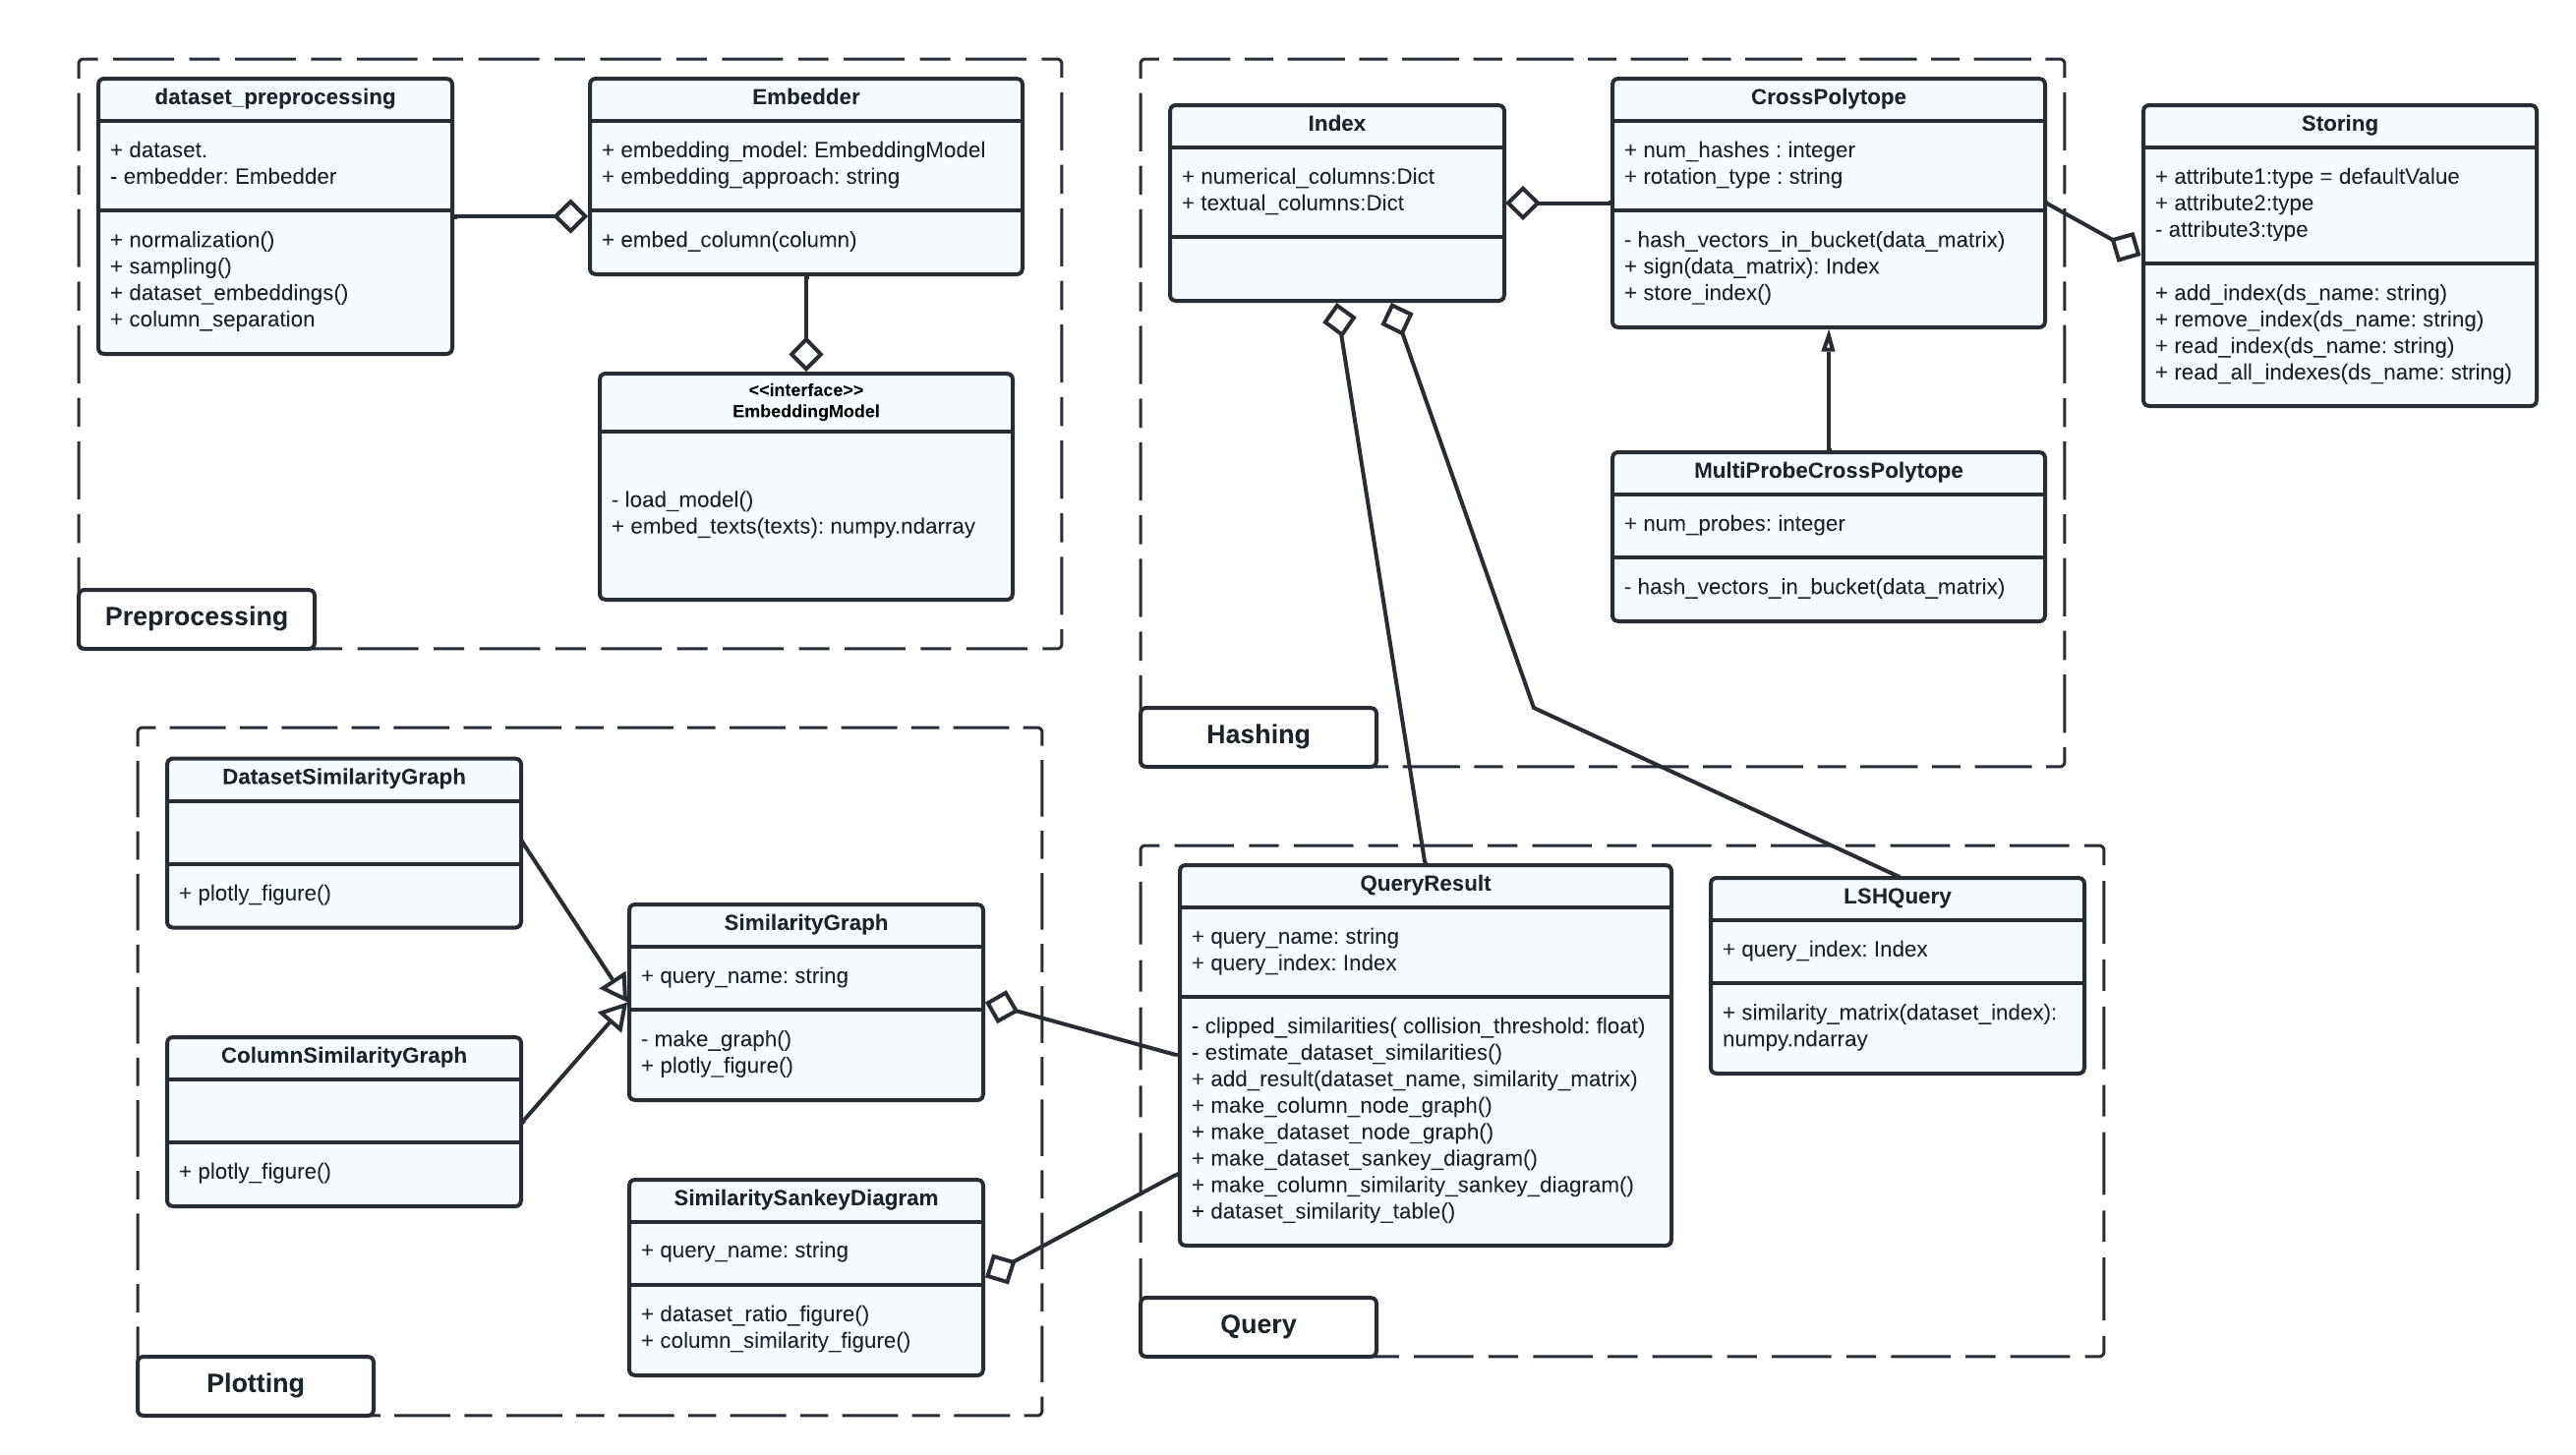
\includegraphics[width=\textwidth]{conception/class-diagram.png}
    \caption{Class Diagram}
    \label{fig:class_diagram}
\end{figure}